\subsection{Ensayo con Carga}

Una vez realizado el ensayo sin carga, y verificado el funcionamiento sin fallas del puente de transistores, se puede proceder a la siguiente prueba. A diferencia del caso anterior, se va a ensayar el convertidor CC-CC completo, conectando el transformador y el inductor de salida $L_f$ a sus terminales correspondientes (ver figura \ref{test_setup}).\\

Como ya se mencionó, la fuente de laboratorio HP 6010A está encargada de proveer la corriente y tensión necesaria en el primario, mientras que la carga electrónica variable ITECH IT8514B+ se conecta en el terminal de salida del secundario y absorbe la corriente continua de la salida. La fuente se configuró en modo de tensión constante (operando a \SI[]{15}{\volt} o \SI[]{30}{\volt}) con limitador de corriente variable, y la carga electrónica en modo de resistencia constante.\\

En esta serie de ensayos se miden distintas variables representativas del sistema: tensión de salida $V_{out}$, tensión rectificada $V_{rect}$, corriente de salida $I_{out}$, corriente en el inductor $I_{Lf}$ y tensión del secundario $V_s$. Como en este caso va a existir circulación de corriente, incluso llegando a cargas cercanas a los \SI[]{100}{\watt} (un tercio de la máxima potencia del sistema), se va a poder observar como se comporta la plataforma frente a grandes circulaciones de corriente, incluido el funcionamiento del rectificador de diodos que no fue evaluado en las pruebas sin carga.\\

\subsubsection{Pruebas a 15 V}

\begin{figure}[h]
    \centering
    %\hspace{0.5em}
    \begin{subfigure}{0.48\textwidth}
        \centering
        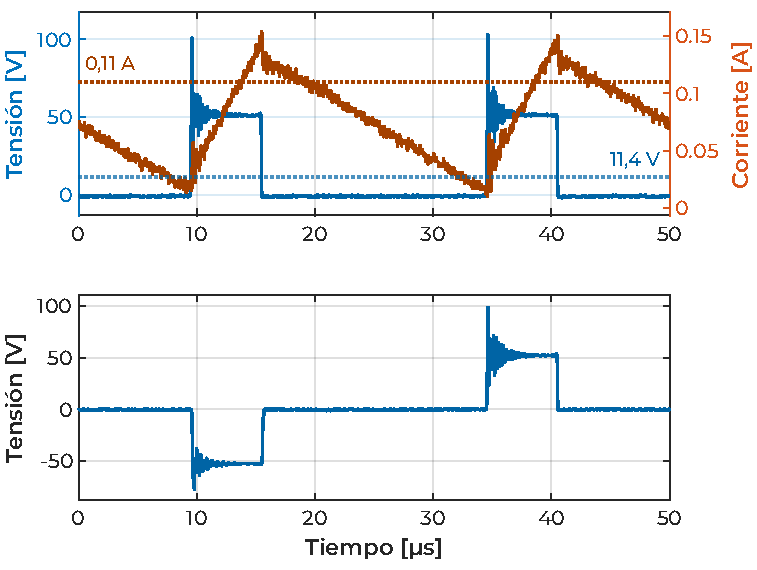
\includegraphics[width=\textwidth]{Imagenes/Con Carga - Caso 3.pdf}
        \caption{Ciclo de trabajo de 25\%.}
        \label{fig:ensayo_concarga15V_DC25}
    \end{subfigure}
    \hspace{0.5em}
    \begin{subfigure}{0.48\textwidth}
        \centering
        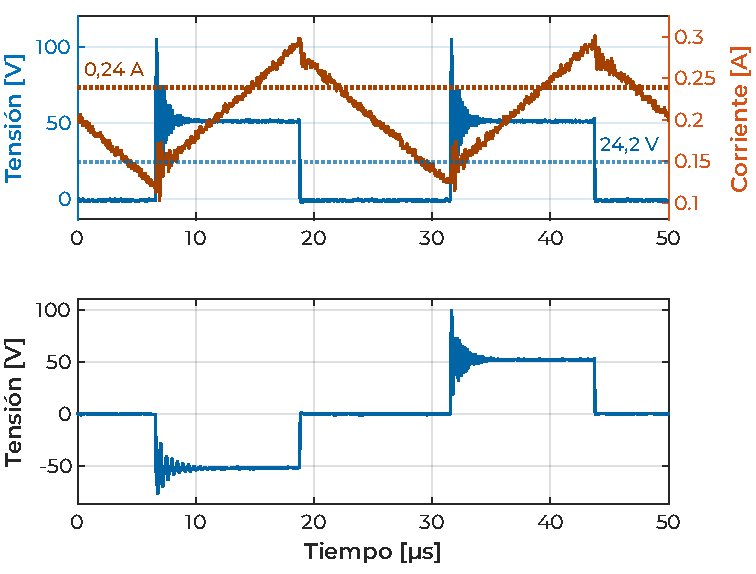
\includegraphics[width=\textwidth]{Imagenes/Con Carga - Caso 1.pdf}
        \caption{Ciclo de trabajo de 50\%.}
        \label{fig:ensayo_concarga15V_DC50}
    \end{subfigure}
    \hfill\vspace{1em}
    \begin{subfigure}{0.48\textwidth}
        \centering
        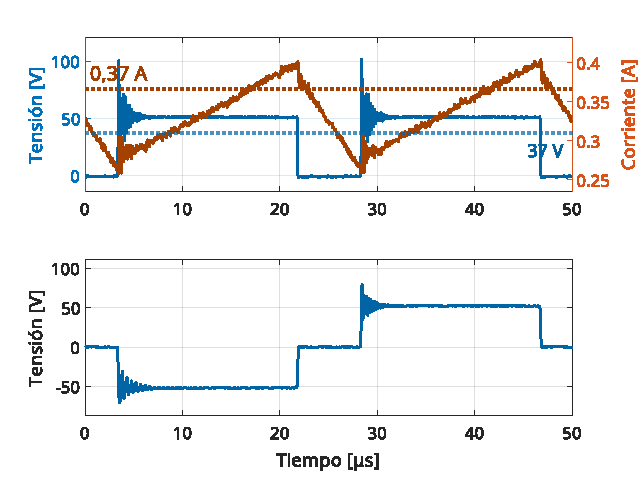
\includegraphics[width=\textwidth]{Imagenes/Con Carga - Caso 5.pdf}
        \caption{Ciclo de trabajo de 75\%.}
        \label{fig:ensayo_concarga15V_DC75}
    \end{subfigure}
    \caption{Tensión rectificada $V_{rect}$, corriente de inductor $I_{Lf}$ y tensión del bobinado secundario $V_{sec}$ para una carga de \SI[]{100}{\ohm} a la salida.}
    \label{fig:ensayo_concarga15V}
\end{figure}

\newpage

Para proteger a los componentes, se comenzaron los ensayos con la fuente de laboratorio entregando una tensión continua de \SI[]{15}{\volt}, limitando la máxima tensión y corriente sobre las llaves y diodos rectificadores. En la figura \ref{fig:ensayo_concarga15V} se pueden apreciar las tensiones y corrientes medidas para tres niveles de ciclo de trabajo $D_{sec}$ distintos (25\%, 50\% y 75\%), todas las medidas tomadas con una carga de \SI[]{100}{\ohm} a la salida. En cada uno de los casos, se presenta la tensión rectificada $V_{rect}$ y la corriente de inductor de salida $I_{Lf}$ en el gráfico superior, y debajo, sincronizada, la tensión del bobinado secundario $V_{sec}$, sin rectificar. Adicionalmente, la fuente y carga variable proveen lecturas numéricas de tensiones, corrientes y potencias de entrada y salida para cada caso (la tensión y corriente de salida se indica en el gráfico con líneas punteadas).\\

En los tres casos, se pueden apreciar los flancos de subida y bajada claramente definidos, obteniendo una onda cuadrada de \SI[]{50}{\volt} en el secundario, con sobrepicos en establecimiento de unos \SI[]{100}{\volt}, correspondientes a los \SI[]{15}{\volt} que ingresan por el primario. Estos sobrepicos son causados por el mismo efecto de ringing del anterior ensayo, solo que se ven amplificados por la circulación de corriente. En tanto a la corriente, se ve claramente la forma triangular de la onda de corriente del inductor $I_{Lf}$, que se carga con una rampa de pendiente positiva cuando circula corriente por el rectificador (semiciclo positivo de la onda $V_{rect}$), y luego se descarga a su valor inicial a través del capacitor y una pata del rectificador, con una rampa de pendiente negativa, manteniendo su valor medio.\\

\subparagraph{Caso A}

Para la figura \ref{fig:ensayo_concarga15V_DC25}, con ciclo de trabajo de 25\%, se obtuvieron \SI[]{11.4}{\volt} de tensión de salida $V_{out}$ con una corriente $I_{out}$ de \SI[]{0.11}{\ampere}, entregando \SI[]{1.25}{\watt} de potencia a la salida. Mientras tanto, a la entrada, con una tensión de \SI[]{15}{\volt} se obtuvo una corriente de entrada $I_{in}$ de \SI[]{0.09}{\ampere}, equivalente a \SI[]{1.35}{\watt} de potencia a la entrada.\\

Esto quiere decir que el convertidor consiguió una marca de eficiencia $\eta$ de alrededor de 92,6\%,comportándose de manera apropiada en condiciones de baja carga, menor al 1\% de la potencia máxima del sistema. Esto se puede notar en la forma de onda de corriente, que se encuentra casi al borde del MCD o \textit{modo de conducción discontinua}, que ocurre cuando el inductor llega a descargarse completamente durante la rampa negativa, y por un período se anula la corriente.\\

\subparagraph{Caso B}

En la figura \ref{fig:ensayo_concarga15V_DC50} se observan los resultados de la prueba ahora con 50\% de ciclo de trabajo. Se obtuvo una tensión de salida de \SI[]{24.2}{\volt} con una corriente de \SI[]{0.24}{\ampere}, resultando en una potencia de salida $P_{out}$ de \SI[]{5.78}{\watt}, más de cuatro veces la potencia del caso anterior. A la entrada circuló una corriente continua de \SI[]{0.42}{\ampere}, entrgándose una potencia de entrada $P_{in}$ de \SI[]{6.30}{\watt}.\\

Esto deriva en una eficiencia energética de 91,7\% para una carga sobre el sistema de aproximadamente 2\%. Al aumentarla carga, la onda de corriente del inductor se alejó del MCD, y presenta una forma triangular con rampas de subida y bajada de pendientes idénticas.\\

\subparagraph{Caso C}

En la figura \ref{fig:ensayo_concarga15V_DC75}, se aumentó el ciclo de trabajo a 75\%, muy próximo al valor máximo establecido en el diseño del transformador. En este caso, se midió una tensión de salida de unos \SI[]{37}{\volt}, correspondiente a una corriente $I_{out}$ de \SI{0.37}{\ampere} y una potencia de \SI[]{13.58}{\watt} entregada a la carga electrónica, más del doble que el caso previo. En la entrada, mientras tanto, se midió una corriente de \SI[]{0.97}{\ampere} que representa una potencia de \SI[]{14.55}{\watt} entregada por la fuente.\\

Haciendo el cálculo, esto significa que en estas condiciones, el sistema logró una eficiencia energética de 93,3\% para una carga de 4,5\%, la más alta medida hasta ahora. En este caso, la pendiente de descarga del inductor es mayor a la de carga, ya que el período de descarga dura una tercera parte del ciclo de carga.\\

\subsubsection{Pruebas a 30 V}

\begin{figure}[h]
    \centering
    \hspace{0.235\textwidth}
    \begin{subfigure}{0.51\textwidth}
        \centering
        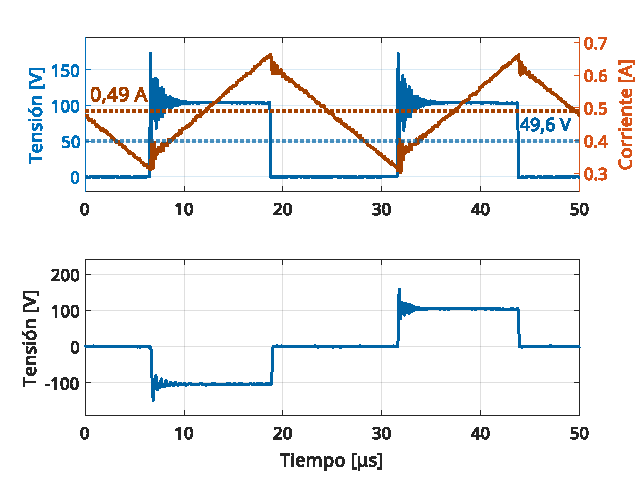
\includegraphics[width=\textwidth]{Imagenes/Con Carga - Caso 7.pdf}
        \caption{Ciclo de trabajo de 50\% y $R_L$ de \SI[]{100}{\ohm}.}
        \label{fig:ensayo_concarga30V_DC50_RL100}
    \end{subfigure}
    \hfill\vspace{1em}
    \begin{subfigure}{0.48\textwidth}
        \centering
        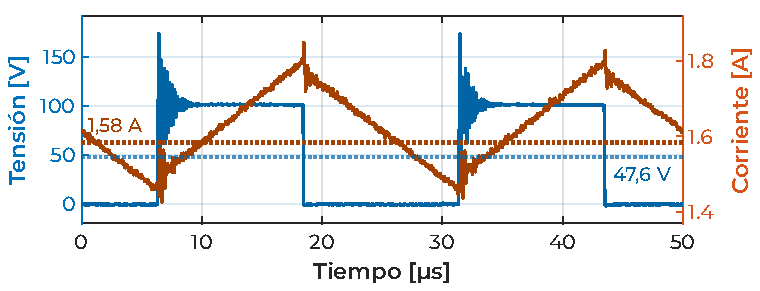
\includegraphics[width=\textwidth]{Imagenes/Con Carga - Caso 9.pdf}
        \caption{Ciclo de trabajo de 50\% y $R_L$ de \SI[]{30}{\ohm}.}
        \label{fig:ensayo_concarga30V_DC50_RL30}
    \end{subfigure}
    \hspace{0.5em}
    \begin{subfigure}{0.48\textwidth}
        \centering
        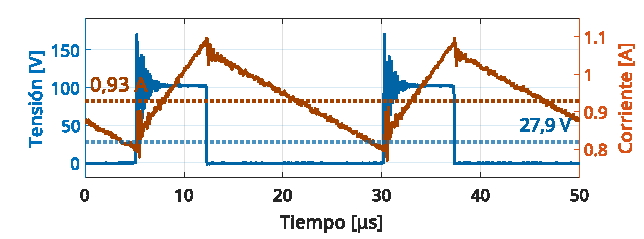
\includegraphics[width=\textwidth]{Imagenes/Con Carga - Caso 10.pdf}
        \caption{Ciclo de trabajo de 25\% y $R_L$ de \SI[]{30}{\ohm}.}
        \label{fig:ensayo_concarga30V_DC25_RL30}
    \end{subfigure}
    \caption{Tensión rectificada $V_{rect}$, corriente de inductor $I_{Lf}$ y tensión del bobinado secundario $V_{sec}$ para distintas condiciones de carga.}
    \label{fig:ensayo_concarga30V}
\end{figure}

Con las pruebas anteriores, con una tensión de entrada de \SI[]{15}{\volt}, nunca se generaron tensiones mayores a \SI[]{100}{\volt}, y las llaves y diodos disiparon una potencia lo suficientemente baja como para no generar una elevación de temperatura perceptible de sus disipadores. Por este motivo, se decidió duplicar la tensión de entrada a \SI[]{30}{\volt}, un valor similar al entregado por la pila de combustible.\\

En la figura \ref{fig:ensayo_concarga30V} se observan las mediciones adquiridas para tres condiciones distintas a \SI[]{30}{\volt} de tensión $V_{in}$: en el primer caso, una resistencia de carga $R_L$ de \SI[]{100}{\ohm} se evalúa con un ciclo de trabajo de 50\%, luego se reduce la resistencia de carga a \SI[]{30}{\ohm} manteniendo $D_{sec}$, y finalmente, manteniendo el nivel de carga, se reduce el ciclo de trabajo a 25\%. En los últimos dos casos se omitió la tensión del bobinado secundario, ya que no aportaba ninguna información adicional.\\

Con este aumento de tensión de entrada, se observa que las ondas cuadradas rectificadas tienen un valor de \SI[]{100}{\volt}, con los efectos de ringing transitorios llegando a niveles elevados de alrededor de \SI[]{200}{\volt}, es decir que presenta sobrepicos del 100\% del valor de establecimiento de la onda cuadrada. Este transitorio tiene una duración ligeramente mayor respecto al ensayo de \SI[]{15}{\volt}, y sus grandes sobrepicos podrían llegar a causar problemas para los diodos. Más adelante se va a proponer una posible solución a implementar para mitigar estos problemas.\\

\subparagraph{Caso A}

En la figura \ref{fig:ensayo_concarga30V_DC50_RL100} se presentan los resultados para una resistencia de carga de \SI[]{100}{\ohm} y un ciclo de trabajo de 50\%, equivalente al caso de la figura \ref{fig:ensayo_concarga15V_DC50} pero con \SI{30}{\volt} a la entrada. Con estas condiciones, se obtuvo una tensión de salida de \SI[]{49.6}{\volt} correspondiente a una corriente sobre la carga de \SI[]{0.49}{\ampere}, que resultan en una potencia de salida $P_{out}$ de \SI[]{24.38}{\watt}. Mientras tanto, a la entrada se inyectó una corriente continua de \SI[]{0.87}{\ampere} que genera una potencia de \SI[]{26.10}{\watt} a la entrada.\\

Estos valores equivalen a una carga del 8\% de la nominal, con una eficiencia energética $\eta$ de 93,4\%, aún mas elevada que el último caso de los ensayos previos. Con estos niveles de potencia, se comenzó a apreciar un muy leve aumento de temperatura en el disipador del rectificador.\\

\subparagraph{Caso B}

En esta prueba de la figura \ref{fig:ensayo_concarga30V_DC50_RL30}, se toman las condiciones anteriores, pero se aumenta significativamente el nivel de carga, reduciendo el valor de $R_L$ a menos de un tercio, \SI[]{30}{\ohm}. Con este cambio, no se percibe una diferencia aprecieble en la tensión rectificada, solo aumentando la magnitud de la corriente. La tensión medida por la carga electrónica a la salida es de \SI[]{47.6}{\volt}, con una corriente $I_{out}$ importante de \SI[]{1.58}{\ampere}, entregando una potencia de \SI[]{75.44}{\watt}. A la entrada, la corriente entregada en los bornes de la pila de combustible es de \SI[]{2.76}{\ampere}, y se genera una potencia de \SI[]{82.80}{\watt}.\\

Con la potencia entregada a la salida, se llega a una carga del 25\% de los \SI[]{300}{\watt} máximos, con una eficiencia de 91,1\%. Este valor bajó ligeramente respecto al caso anterior, indicando algún tipo de pérdida resistiva que aumenta con la corriente. Además, con este nivel de carga se comienza a apreciar más la elevación de temperatura de ambos disipadores.\\

\subparagraph{Caso C}

Finalmente, se realizó el ultimo ensayo (figura \ref{fig:ensayo_concarga30V_DC25_RL30}), con el mismo nivel de carga de \SI[]{30}{\ohm} pero un ciclo de trabajo de 25\%. Con esta configuración, se obtuvieron \SI[]{25.93}{\watt} a la salida, con una corriente de \SI[]{0.93}{\ampere} a una tensión de \SI[]{27.9}{\volt}. En la entrada del primario, fue inyectada una potencia de \SI[]{28.8}{\watt} por medio de una corriente $I_{in}$ de \SI[]{0.96}{\ampere}. Esta configuración del sistema da una eficiencia energética del 90\% para una carga total de 8,6\%.\\

\subsubsection{Efecto de Ringing}

Este efecto de ringing que se presenta en todos los flancos de subida, en particular para altas corrientes, es problemático ya que genera sobrepicos de tensión muy elevados que pueden dañar los componentes, además de empeorar el rendimiento y eficiencia energética del convertidor. Este efecto se presenta generalmente en sistemas con cargas inductivas: cuando se corta la repentinamente una alta circulación de corriente (como es el caso de las llaves y diodos), se genera una fuerza contra-electromotriz que se opone al cambio de corriente, y que causa los picos de tensión sobre las llaves y la oscilación subamortiguada.\\

\begin{figure}[h]
    \centering
    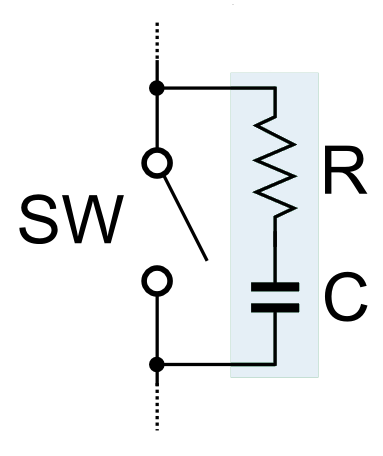
\includegraphics[scale=0.2]{Imagenes/Snubber RC.png}
    \caption{Circuito snubber RC en paralelo a una llave, para mitigar el efecto de ringing inductivo.}
    \label{snubber_rc}
\end{figure}

Para mitigar este problema, se puede implementar un circuito RC serie llamado \textit{snubber}, conectado en paralelo a las llaves y transistores, que provee un camino alternativo de corta duración (hasta que se cargue el capacitor) para la corriente de descarga de los elementos inductivos (ver figura \ref{snubber_rc}). Al diseñar la placa se tuvo en cuenta este efecto, y se dejaron footprints para poder agregar un circuito snubber a cada llave y diodo en caso de ser necesario.\\